\documentclass{beamer}
\usepackage{graphicx} % Required for inserting images
\usepackage{amsmath}

\title{Domača naloga 1}
\author{Urban Zgonc}
\date{November 2024} 

\begin{document}

\maketitle

\begin{frame}{Kazalo}

\begin{itemize}
\item 1. naloga
\item 2. naloga
\item 3. naloga
\end{itemize}


\end{frame}


\begin{frame}{1. naloga}

\begin{itemize}
    \item  Dobili smo datoteko "naloga1-1.txt",
    \item  V prvi vrstici je podana količina in enota podatkov: time[s],
    \item  V drugi vrstici je podano število podatkov in pa število podatkov v vrstici,
    \item  V naslednjih stotih vrsticah je podan čas od 0 do 1 sekunde, 
    \item  Datoteko smo prebrali s funkcijo importdata, v katero smo vstavili ime datoteke in pa koliko prvih vrstic naj funkcija ne prebere,
    \item  Vse prebrane podatke iz datoteke smo shranili v vektor t
\end{itemize}  

\end{frame}


\begin{frame}{2. naloga}

\begin{itemize}
    \item  Graf moči v odvisnosti od časa:
\end{itemize}  

\begin{figure}
    \centering
    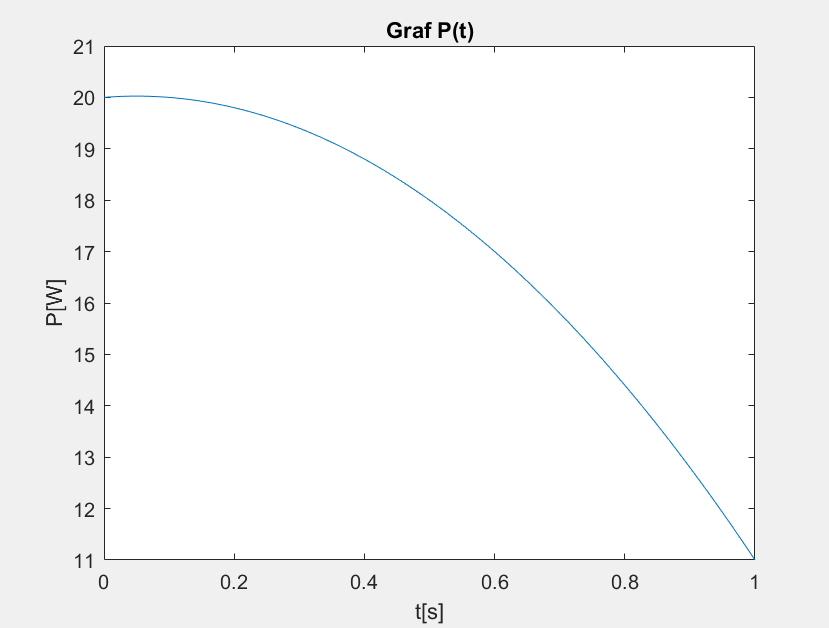
\includegraphics[width=1\linewidth]{image.png}
    \caption{Graf moči v odvisnosti od časa}
    \label{fig:enter-label}
\end{figure}

\end{frame}

\begin{frame}
\frametitle{3. naloga}

Trapezna formula za numerično integracijo funkcije \( f(x) \) na intervalu \([a, b]\) je podano z naslednjo enačbo:

\[
\int_a^b f(x) \, dx = \frac{\Delta x}{2} \left( f(x_0) + 2f(x_1) + 2f(x_2) + \dots + 2f(x_{n-1}) + f(x_n) \right)
\]

Rezultat integrala: 17.166497

\end{frame}

\end{document}
